\section{Preliminary Study}

% vim: ft=tex
%!TEX root=../icsme2016-mrstudyr.tex

\begin{table}[t!]
  % \vspace{-0.75em}
    \caption{Schemas analysed in the empirical study.}\label{tbl:study-schemas}
  \vspace{-1em}
  \footnotesize
  \centering
  \scalebox{\tablescalefactor}{
    \begin{tabular}{l@{\hskip -5pt}rrrrrrrr}
      {Schema} & \rot{Tables} & \rot{Columns} & \rot{Checks} & \rot{Foreign Keys} & \rot{Not Nulls} & \rot{Primary Keys} & \rot{Uniques} & \rot{$\sum$Constraints} \\
      \toprule

      CoffeeOrders & 5 & 20 & 0 & 4 & 10 & 5 & 0 & 19 \\
      Employee & 1 & 7 & 3 & 0 & 0 & 1 & 0 & 4 \\
      Inventory & 1 & 4 & 0 & 0 & 0 & 1 & 1 & 2 \\
      Iso3166 & 1 & 3 & 0 & 0 & 2 & 1 & 0 & 3 \\
      JWhoisServer & 6 & 49 & 0 & 0 & 44 & 6 & 0 & 50 \\
      MozillaPermissions & 1 & 8 & 0 & 0 & 0 & 1 & 0 & 1 \\
      NistWeather & 2 & 9 & 5 & 1 & 5 & 2 & 0 & 13 \\
      Person & 1 & 5 & 1 & 0 & 5 & 1 & 0 & 7 \\
      Products & 3 & 9 & 4 & 2 & 5 & 3 & 0 & 14 \\
      \midrule
      Total & 21 & 114 & 13 & 7 & 71 & 21 & 1 & 113 \\

      \bottomrule
    \end{tabular}
  }
  \vspace{-1em}
\end{table}


% GMK NOTE: All of this content is really about the design of the experiments and thus it has to be integrated into this
% section (currently, this is still rough content).

We chose these nine schemas because they range in triviality. For example, the MozillaPermissions schema contains a
single constraint, where as the JWhoisServer schema has a total of 50 constraints. This allowed us to evaluate the
policy recommendations made based on the effectiveness of reduction techniques analysed by \mr~for schemas of varying
complexities.

Where Wong and Mathur in their studies~\cite{mathur1994empirical, wong1993mutation} conducted experiments using mutant
sampling with $x$ from $10\%$ to $40\%$ increasing by steps of $5\%$, we chose to analyse $x$ at $1\%$ and then increase
by $10\%$ intervals up to $90\%$. By lowering the granularity of the experiment to $10\%$ intervals instead of $1\%$ or
$5\%$, we reduce the cost of performing retrospective analysis with \mr, while observing similar trends.

\hspace*{-1em}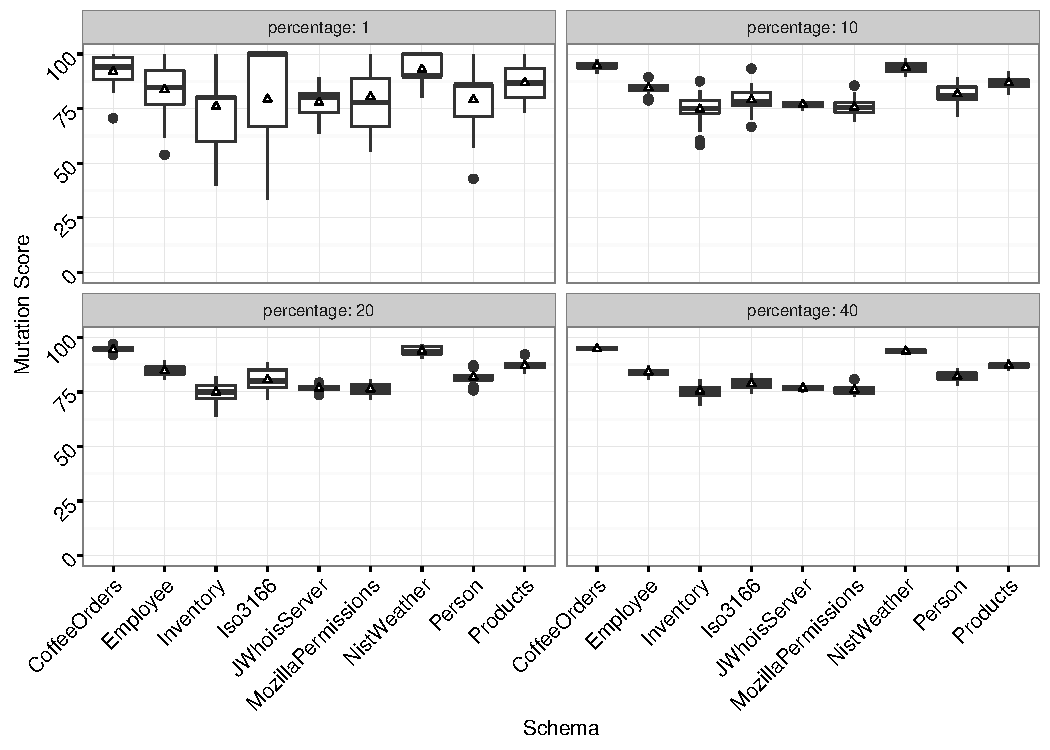
\includegraphics[scale = 0.5]{graphs/schema_vs_ms.pdf}
